\chapter{Background and Related Work}
\label{bg}
% \SVN $Revision: 838 $
% \SVN $Author: sgordon $
% \SVN $Date: 2014-05-12 13:30:42 +0700 (Mon, 12 May 2014) $
% \SVN $URL: https://sandilands.info/svn/Common/Styles/siitthesis/chapter2.tex $

Recently, wireless networking are witnessing several deployments in various extreme environments where they usually suffer from different levels of link disruptions depending on the severity of the operations. 
Commonly, these networks are known as Intermittently Connected Networks (ICNs). 
An ICNs, also known as a Challenged Network, is an infrastructure-less wireless network that supports the proper functionality of the wireless applications operating in stressful environments, where excessive delays and no existence of end-to-end path(s) between any arbitrary source-destination pair, result from highly repetitive link disruptions \cite{Khabbaz2012}.
In order to handle ICNs, the Internet Engineering Task Force (IETF) \cite{Cerf2007} proposed an architecture called Delay-/Disruption-Tolerant Networks (DTNs).
DTNs can basically be categorized into 3 types: scheduled networks, predictable networks and opportunistic networks.
In this thesis, we focus on the research on the most extreme case of DTNs which is the opportunistic networks.

This chapter gives the background knowledge of this thesis. 
The background of Delay Tolerant Networks is presented in Section~\ref{bg:Delay Tolerant Networks}. 
Additionally, an explanation of Opportunistic Networks is presented in Section~\ref{bg:Opportunistic Networks}. 
%=============================================================================
\section{Delay Tolerant Networks}
\label{bg:Delay Tolerant Networks}
%=============================================================================
DTNs is an overlay architecture with an aim to operate over the protocol stacks of the ICNs and enable gateway functionality between them through the use of storage capacity, a variety of protocol techniques, replication and parallel forwarding, forward error correction and many other techniques for overcoming the impairments of communication  \cite{Khabbaz2012}.
DTNs enable the transferring of data in extremely challenging environments where networks are assumed to experience frequent, long-duration partitioning and may have no end-to-end connectivity between source and destination \cite{Liu2011}. 
Therefore, the timer and acknowledgement mechanisms of the traditional TCP/IP protocol definitely fail in such circumstances \cite{Souza2010}.
In addition, the routing algorithms designed for Mobile Ad hoc NETworks (MANETs) can not perform effectively under aforementioned constraints as well, since the availability of contemporaneous end-to-end connectivity is essential for conventional routing algorithms \cite{Yue2013}.

Basically the types of DTNs can be classified in 3 categories: scheduled networks, predictable networks and opportunistic networks as seen in Figure~\ref{fig:bg:Type of DTN}.
In DTNs, predictable and scheduled networks are the common aim in designing the routing protocols in the highly disruptive environments such as Interplanetary Internet (IPN) \cite{Burleigh2003} where the contact time is not completely random but in periodic interval.
In the thesis, we study in the most extreme case of DTNs which is the opportunistic networks where the contact time is undetermined along with stochastic movements.


\begin{figure}
\centering
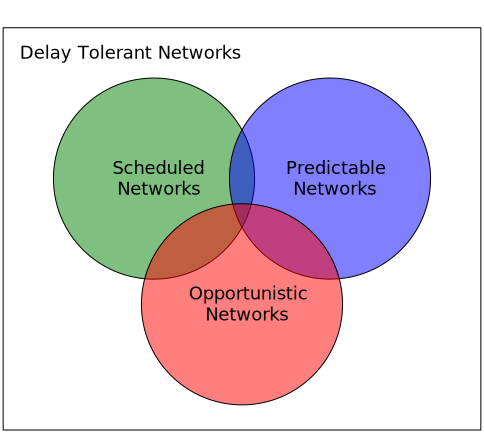
\includegraphics[width=0.5\columnwidth]{Figures/TypeOfDTN.pdf}
\caption{Types of DTN}
\label{fig:bg:Type of DTN}
\end{figure} 


%=============================================================================
\section{Opportunistic Networks}
\label{bg:Opportunistic Networks}
%=============================================================================
In fact, Opportunistic networks focus on mobile ad-hoc DTNs, where tolerant delayed routes between the source and destination are built dynamically.
However, OppNets is different from MANETs that it does not assume the existing end-to-end connectivity.
Therefore, instead of depending on end-to-end MANETs routing protocols, the messages are delivered through one hop data transmission among opportunistic node encounters with intermediate node storage and mobility, called \textit{Store-Carry-Forward paradigm} \cite{Hu2009}. 
In essential, there are three common steps of routing in OppNet \cite{Hsu2011}:
\begin{itemize}
	\item Broadcast the messages to candicate relayed nodes.
	\item Select the best candidate node.
	\item Forward the messages.
\end{itemize}



%=============================================================================
\subsection{Opportunistic Routing}
\label{bg:Opportunistic Networks:Opportunistic Routing}
%=============================================================================
In this opportunistic routing, the nodes can exchange data in a spontaneous manner whenever they come in close.
If there is no direct connection from source to destination, data holding nodes will discover their nearest neighbor nodes to forward messages toward the destination node.
Thus, this opportunistic route is determined at each hop when messages traverse through different hops.
In this routing scheme, mobile nodes are normally equipped with local knowledge of the best nodes around them to determine the best path to transmit the messages with this knowledge.
In the case of such nodes absence, the node currently holding the message simply stores the messages and wait for an opportunity to forward the packets.
This  infrastructure-less wireless network environment requires common 2 factors to facilitate the opportunistic routing \cite{Poonguzharselvi2013a} : 
\begin{itemize}
	\item Destination path finding:
	Intermediate nodes are used to form paths dynamically since there is no fixed path from source to destination nodes.
	\item Next hop forwarder selection:
	Data holding nodes need to find a helper node that can forward the messages to the destination as soon as possible.
\end{itemize}


%=============================================================================
\subsection{Classification of Opportunistic Routing}
\label{bg:Opportunistic Networks:Classification of Opportunistic Routing}
%=============================================================================

Several researches proposed opportunistic routing algorithms based on store-carry-forward mechanism.
The existing common OR algorithms can be classified based on their data forwarding behavior as shown in Figure \ref{fig:bg:RoutingInOppNets} 
% \begin{figure}
% 	\centering
% 	\includegraphics[width=1.0\columnwidth]{Figures/RoutingInOppNets.pdf}
% 	\caption{Classification of Opportunistic Routing}
% 	\label{fig:bg:RoutingInOppNets}
% \end{figure}

%% This part is folding for OppNet routing diagram
\begin{figure}
	\centering
%%SpaceForGraphic
% Graphic for TeX using PGF
% Title: /Users/Arm/Desktop/Diagram1.dia
% Creator: Dia v0.97.2
% CreationDate: Thu Sep 11 22:05:10 2014
% For: Arm
% \usepackage{tikz}
% The following commands are not supported in PSTricks at present
% We define them conditionally, so when they are implemented,
% this pgf file will use them.
\ifx\du\undefined
  \newlength{\du}
\fi
\setlength{\du}{15\unitlength}
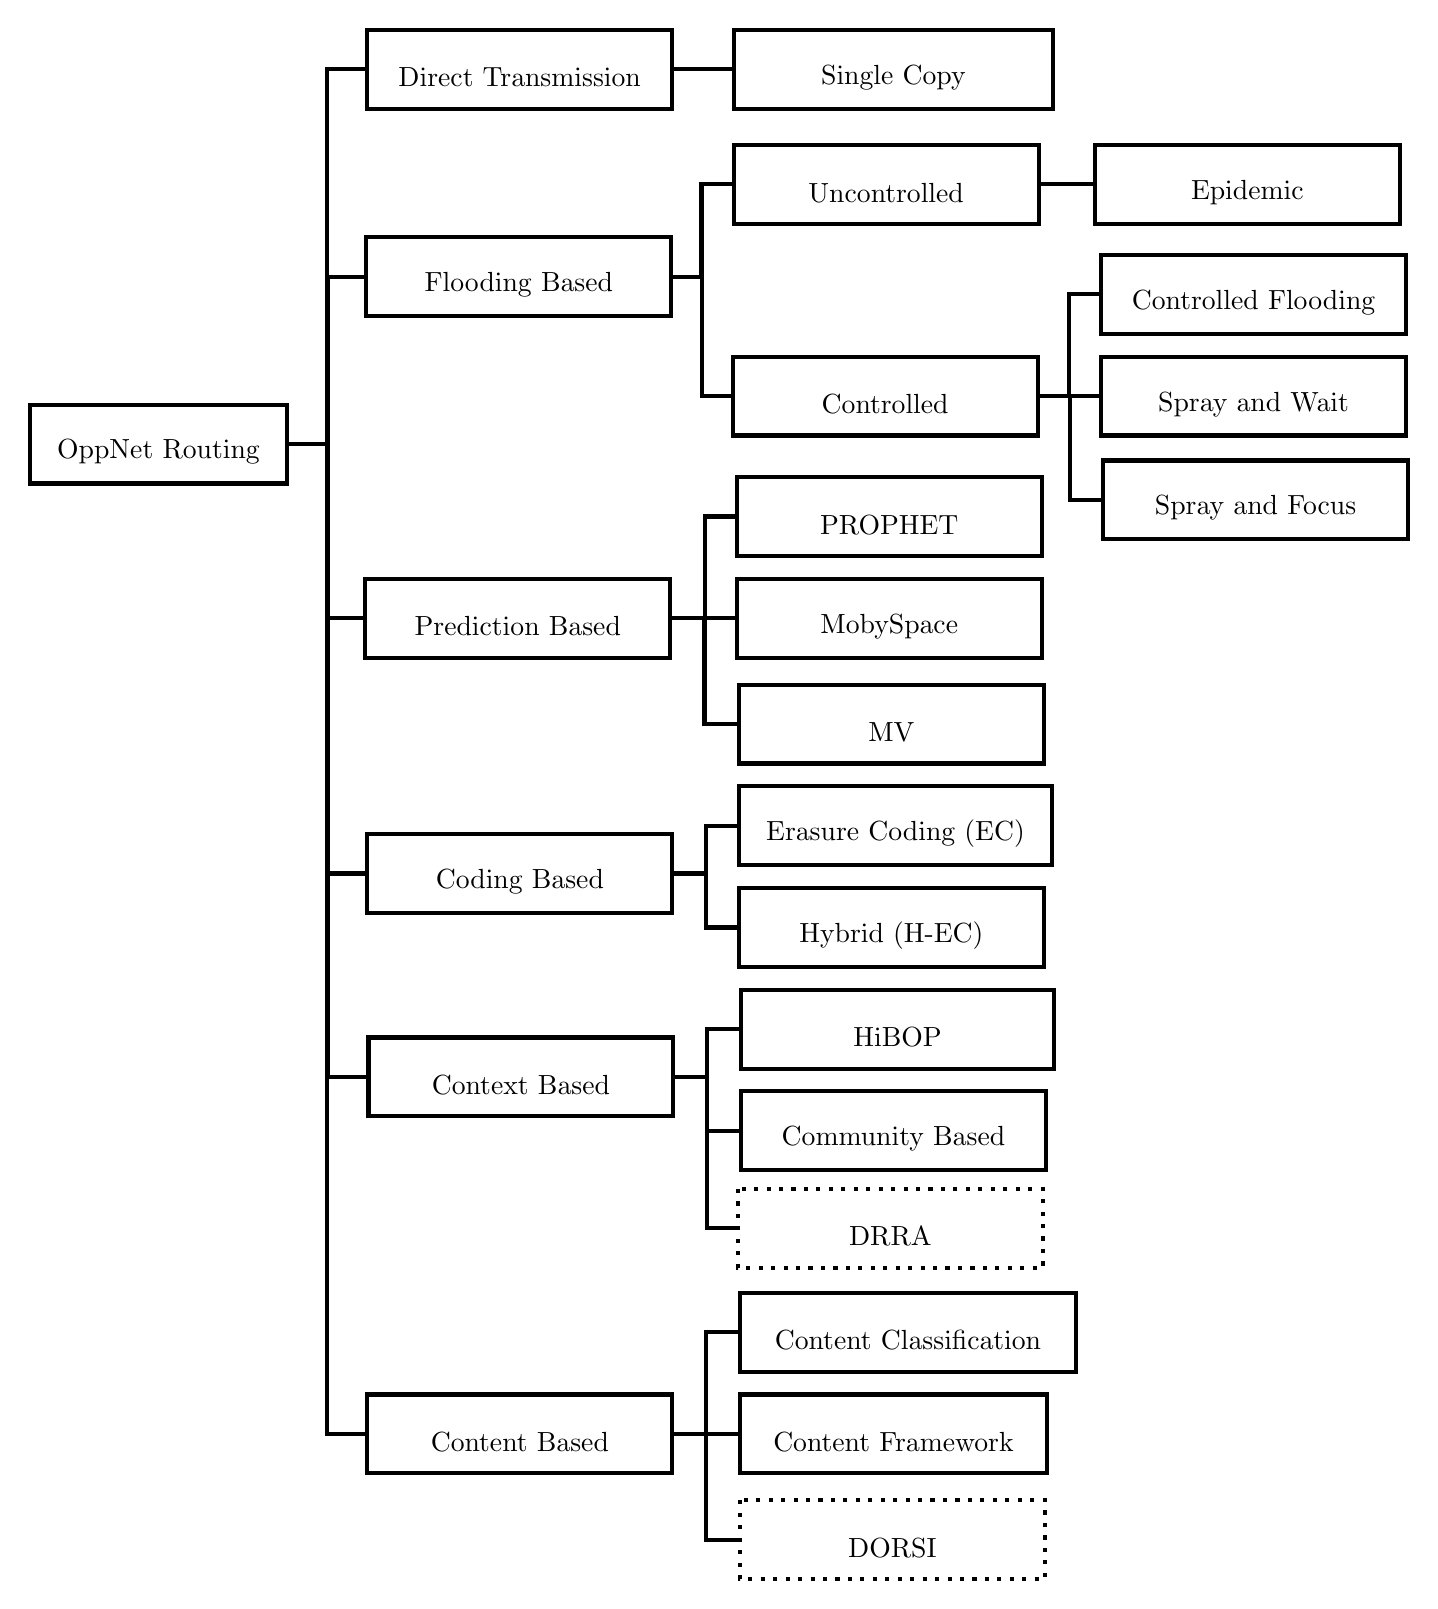
\begin{tikzpicture}
\pgftransformxscale{1.000000}
\pgftransformyscale{-1.000000}
\definecolor{dialinecolor}{rgb}{0.000000, 0.000000, 0.000000}
\pgfsetstrokecolor{dialinecolor}
\definecolor{dialinecolor}{rgb}{1.000000, 1.000000, 1.000000}
\pgfsetfillcolor{dialinecolor}
\definecolor{dialinecolor}{rgb}{1.000000, 1.000000, 1.000000}
\pgfsetfillcolor{dialinecolor}
\fill (3.606250\du,23.050000\du)--(3.606250\du,24.950000\du)--(9.808750\du,24.950000\du)--(9.808750\du,23.050000\du)--cycle;
\pgfsetlinewidth{0.100000\du}
\pgfsetdash{}{0pt}
\pgfsetdash{}{0pt}
\pgfsetmiterjoin
\definecolor{dialinecolor}{rgb}{0.000000, 0.000000, 0.000000}
\pgfsetstrokecolor{dialinecolor}
\draw (3.606250\du,23.050000\du)--(3.606250\du,24.950000\du)--(9.808750\du,24.950000\du)--(9.808750\du,23.050000\du)--cycle;
% setfont left to latex
\definecolor{dialinecolor}{rgb}{0.000000, 0.000000, 0.000000}
\pgfsetstrokecolor{dialinecolor}
\node at (6.707500\du,24.195000\du){OppNet Routing};
\definecolor{dialinecolor}{rgb}{1.000000, 1.000000, 1.000000}
\pgfsetfillcolor{dialinecolor}
\fill (11.736200\du,14.020000\du)--(11.736200\du,15.920000\du)--(19.081200\du,15.920000\du)--(19.081200\du,14.020000\du)--cycle;
\pgfsetlinewidth{0.100000\du}
\pgfsetdash{}{0pt}
\pgfsetdash{}{0pt}
\pgfsetmiterjoin
\definecolor{dialinecolor}{rgb}{0.000000, 0.000000, 0.000000}
\pgfsetstrokecolor{dialinecolor}
\draw (11.736200\du,14.020000\du)--(11.736200\du,15.920000\du)--(19.081200\du,15.920000\du)--(19.081200\du,14.020000\du)--cycle;
% setfont left to latex
\definecolor{dialinecolor}{rgb}{0.000000, 0.000000, 0.000000}
\pgfsetstrokecolor{dialinecolor}
\node at (15.408700\du,15.165000\du){Direct Transmission};
\pgfsetlinewidth{0.100000\du}
\pgfsetdash{}{0pt}
\pgfsetdash{}{0pt}
\pgfsetmiterjoin
\pgfsetbuttcap
{
\definecolor{dialinecolor}{rgb}{0.000000, 0.000000, 0.000000}
\pgfsetfillcolor{dialinecolor}
% was here!!!
{\pgfsetcornersarced{\pgfpoint{0.000000\du}{0.000000\du}}\definecolor{dialinecolor}{rgb}{0.000000, 0.000000, 0.000000}
\pgfsetstrokecolor{dialinecolor}
\draw (9.859135\du,24.000000\du)--(10.772440\du,24.000000\du)--(10.772440\du,14.970000\du)--(11.685746\du,14.970000\du);
}}
\definecolor{dialinecolor}{rgb}{1.000000, 1.000000, 1.000000}
\pgfsetfillcolor{dialinecolor}
\fill (20.574100\du,14.020000\du)--(20.574100\du,15.920000\du)--(28.250804\du,15.920000\du)--(28.250804\du,14.020000\du)--cycle;
\pgfsetlinewidth{0.100000\du}
\pgfsetdash{}{0pt}
\pgfsetdash{}{0pt}
\pgfsetmiterjoin
\definecolor{dialinecolor}{rgb}{0.000000, 0.000000, 0.000000}
\pgfsetstrokecolor{dialinecolor}
\draw (20.574100\du,14.020000\du)--(20.574100\du,15.920000\du)--(28.250804\du,15.920000\du)--(28.250804\du,14.020000\du)--cycle;
% setfont left to latex
\definecolor{dialinecolor}{rgb}{0.000000, 0.000000, 0.000000}
\pgfsetstrokecolor{dialinecolor}
\node at (24.412452\du,15.165000\du){Single Copy};
\pgfsetlinewidth{0.100000\du}
\pgfsetdash{}{0pt}
\pgfsetdash{}{0pt}
\pgfsetmiterjoin
\pgfsetbuttcap
{
\definecolor{dialinecolor}{rgb}{0.000000, 0.000000, 0.000000}
\pgfsetfillcolor{dialinecolor}
% was here!!!
{\pgfsetcornersarced{\pgfpoint{0.000000\du}{0.000000\du}}\definecolor{dialinecolor}{rgb}{0.000000, 0.000000, 0.000000}
\pgfsetstrokecolor{dialinecolor}
\draw (19.131654\du,14.970000\du)--(19.181654\du,14.970000\du)--(20.473625\du,14.970000\du)--(20.523625\du,14.970000\du);
}}
\definecolor{dialinecolor}{rgb}{1.000000, 1.000000, 1.000000}
\pgfsetfillcolor{dialinecolor}
\fill (11.715000\du,19.020000\du)--(11.715000\du,20.920000\du)--(19.060000\du,20.920000\du)--(19.060000\du,19.020000\du)--cycle;
\pgfsetlinewidth{0.100000\du}
\pgfsetdash{}{0pt}
\pgfsetdash{}{0pt}
\pgfsetmiterjoin
\definecolor{dialinecolor}{rgb}{0.000000, 0.000000, 0.000000}
\pgfsetstrokecolor{dialinecolor}
\draw (11.715000\du,19.020000\du)--(11.715000\du,20.920000\du)--(19.060000\du,20.920000\du)--(19.060000\du,19.020000\du)--cycle;
% setfont left to latex
\definecolor{dialinecolor}{rgb}{0.000000, 0.000000, 0.000000}
\pgfsetstrokecolor{dialinecolor}
\node at (15.387500\du,20.165000\du){Flooding Based};
\definecolor{dialinecolor}{rgb}{1.000000, 1.000000, 1.000000}
\pgfsetfillcolor{dialinecolor}
\fill (20.565000\du,16.795000\du)--(20.565000\du,18.695000\du)--(27.910000\du,18.695000\du)--(27.910000\du,16.795000\du)--cycle;
\pgfsetlinewidth{0.100000\du}
\pgfsetdash{}{0pt}
\pgfsetdash{}{0pt}
\pgfsetmiterjoin
\definecolor{dialinecolor}{rgb}{0.000000, 0.000000, 0.000000}
\pgfsetstrokecolor{dialinecolor}
\draw (20.565000\du,16.795000\du)--(20.565000\du,18.695000\du)--(27.910000\du,18.695000\du)--(27.910000\du,16.795000\du)--cycle;
% setfont left to latex
\definecolor{dialinecolor}{rgb}{0.000000, 0.000000, 0.000000}
\pgfsetstrokecolor{dialinecolor}
\node at (24.237500\du,17.940000\du){Uncontrolled};
\definecolor{dialinecolor}{rgb}{1.000000, 1.000000, 1.000000}
\pgfsetfillcolor{dialinecolor}
\fill (20.540000\du,21.895000\du)--(20.540000\du,23.795000\du)--(27.885000\du,23.795000\du)--(27.885000\du,21.895000\du)--cycle;
\pgfsetlinewidth{0.100000\du}
\pgfsetdash{}{0pt}
\pgfsetdash{}{0pt}
\pgfsetmiterjoin
\definecolor{dialinecolor}{rgb}{0.000000, 0.000000, 0.000000}
\pgfsetstrokecolor{dialinecolor}
\draw (20.540000\du,21.895000\du)--(20.540000\du,23.795000\du)--(27.885000\du,23.795000\du)--(27.885000\du,21.895000\du)--cycle;
% setfont left to latex
\definecolor{dialinecolor}{rgb}{0.000000, 0.000000, 0.000000}
\pgfsetstrokecolor{dialinecolor}
\node at (24.212500\du,23.040000\du){Controlled};
\definecolor{dialinecolor}{rgb}{1.000000, 1.000000, 1.000000}
\pgfsetfillcolor{dialinecolor}
\fill (29.265000\du,16.795000\du)--(29.265000\du,18.695000\du)--(36.610000\du,18.695000\du)--(36.610000\du,16.795000\du)--cycle;
\pgfsetlinewidth{0.100000\du}
\pgfsetdash{}{0pt}
\pgfsetdash{}{0pt}
\pgfsetmiterjoin
\definecolor{dialinecolor}{rgb}{0.000000, 0.000000, 0.000000}
\pgfsetstrokecolor{dialinecolor}
\draw (29.265000\du,16.795000\du)--(29.265000\du,18.695000\du)--(36.610000\du,18.695000\du)--(36.610000\du,16.795000\du)--cycle;
% setfont left to latex
\definecolor{dialinecolor}{rgb}{0.000000, 0.000000, 0.000000}
\pgfsetstrokecolor{dialinecolor}
\node at (32.937500\du,17.940000\du){Epidemic};
\pgfsetlinewidth{0.100000\du}
\pgfsetdash{}{0pt}
\pgfsetdash{}{0pt}
\pgfsetmiterjoin
\pgfsetbuttcap
{
\definecolor{dialinecolor}{rgb}{0.000000, 0.000000, 0.000000}
\pgfsetfillcolor{dialinecolor}
% was here!!!
{\pgfsetcornersarced{\pgfpoint{0.000000\du}{0.000000\du}}\definecolor{dialinecolor}{rgb}{0.000000, 0.000000, 0.000000}
\pgfsetstrokecolor{dialinecolor}
\draw (9.859135\du,24.000000\du)--(10.787067\du,24.000000\du)--(10.787067\du,19.970000\du)--(11.715000\du,19.970000\du);
}}
\pgfsetlinewidth{0.100000\du}
\pgfsetdash{}{0pt}
\pgfsetdash{}{0pt}
\pgfsetmiterjoin
\pgfsetbuttcap
{
\definecolor{dialinecolor}{rgb}{0.000000, 0.000000, 0.000000}
\pgfsetfillcolor{dialinecolor}
% was here!!!
{\pgfsetcornersarced{\pgfpoint{0.000000\du}{0.000000\du}}\definecolor{dialinecolor}{rgb}{0.000000, 0.000000, 0.000000}
\pgfsetstrokecolor{dialinecolor}
\draw (19.060000\du,19.970000\du)--(19.787273\du,19.970000\du)--(19.787273\du,17.745000\du)--(20.514546\du,17.745000\du);
}}
\pgfsetlinewidth{0.100000\du}
\pgfsetdash{}{0pt}
\pgfsetdash{}{0pt}
\pgfsetmiterjoin
\pgfsetbuttcap
{
\definecolor{dialinecolor}{rgb}{0.000000, 0.000000, 0.000000}
\pgfsetfillcolor{dialinecolor}
% was here!!!
{\pgfsetcornersarced{\pgfpoint{0.000000\du}{0.000000\du}}\definecolor{dialinecolor}{rgb}{0.000000, 0.000000, 0.000000}
\pgfsetstrokecolor{dialinecolor}
\draw (19.110454\du,19.970000\du)--(19.800000\du,19.970000\du)--(19.800000\du,22.845000\du)--(20.489546\du,22.845000\du);
}}
\pgfsetlinewidth{0.100000\du}
\pgfsetdash{}{0pt}
\pgfsetdash{}{0pt}
\pgfsetmiterjoin
\pgfsetbuttcap
{
\definecolor{dialinecolor}{rgb}{0.000000, 0.000000, 0.000000}
\pgfsetfillcolor{dialinecolor}
% was here!!!
{\pgfsetcornersarced{\pgfpoint{0.000000\du}{0.000000\du}}\definecolor{dialinecolor}{rgb}{0.000000, 0.000000, 0.000000}
\pgfsetstrokecolor{dialinecolor}
\draw (27.960454\du,17.745000\du)--(28.010454\du,17.745000\du)--(29.164546\du,17.745000\du)--(29.214546\du,17.745000\du);
}}
\definecolor{dialinecolor}{rgb}{1.000000, 1.000000, 1.000000}
\pgfsetfillcolor{dialinecolor}
\fill (29.415000\du,19.445000\du)--(29.415000\du,21.345000\du)--(36.760000\du,21.345000\du)--(36.760000\du,19.445000\du)--cycle;
\pgfsetlinewidth{0.100000\du}
\pgfsetdash{}{0pt}
\pgfsetdash{}{0pt}
\pgfsetmiterjoin
\definecolor{dialinecolor}{rgb}{0.000000, 0.000000, 0.000000}
\pgfsetstrokecolor{dialinecolor}
\draw (29.415000\du,19.445000\du)--(29.415000\du,21.345000\du)--(36.760000\du,21.345000\du)--(36.760000\du,19.445000\du)--cycle;
% setfont left to latex
\definecolor{dialinecolor}{rgb}{0.000000, 0.000000, 0.000000}
\pgfsetstrokecolor{dialinecolor}
\node at (33.087500\du,20.590000\du){Controlled Flooding};
\definecolor{dialinecolor}{rgb}{1.000000, 1.000000, 1.000000}
\pgfsetfillcolor{dialinecolor}
\fill (29.415000\du,21.895000\du)--(29.415000\du,23.795000\du)--(36.760000\du,23.795000\du)--(36.760000\du,21.895000\du)--cycle;
\pgfsetlinewidth{0.100000\du}
\pgfsetdash{}{0pt}
\pgfsetdash{}{0pt}
\pgfsetmiterjoin
\definecolor{dialinecolor}{rgb}{0.000000, 0.000000, 0.000000}
\pgfsetstrokecolor{dialinecolor}
\draw (29.415000\du,21.895000\du)--(29.415000\du,23.795000\du)--(36.760000\du,23.795000\du)--(36.760000\du,21.895000\du)--cycle;
% setfont left to latex
\definecolor{dialinecolor}{rgb}{0.000000, 0.000000, 0.000000}
\pgfsetstrokecolor{dialinecolor}
\node at (33.087500\du,23.040000\du){Spray and Wait};
\definecolor{dialinecolor}{rgb}{1.000000, 1.000000, 1.000000}
\pgfsetfillcolor{dialinecolor}
\fill (29.465000\du,24.395000\du)--(29.465000\du,26.295000\du)--(36.810000\du,26.295000\du)--(36.810000\du,24.395000\du)--cycle;
\pgfsetlinewidth{0.100000\du}
\pgfsetdash{}{0pt}
\pgfsetdash{}{0pt}
\pgfsetmiterjoin
\definecolor{dialinecolor}{rgb}{0.000000, 0.000000, 0.000000}
\pgfsetstrokecolor{dialinecolor}
\draw (29.465000\du,24.395000\du)--(29.465000\du,26.295000\du)--(36.810000\du,26.295000\du)--(36.810000\du,24.395000\du)--cycle;
% setfont left to latex
\definecolor{dialinecolor}{rgb}{0.000000, 0.000000, 0.000000}
\pgfsetstrokecolor{dialinecolor}
\node at (33.137500\du,25.540000\du){Spray and Focus};
\pgfsetlinewidth{0.100000\du}
\pgfsetdash{}{0pt}
\pgfsetdash{}{0pt}
\pgfsetmiterjoin
\pgfsetbuttcap
{
\definecolor{dialinecolor}{rgb}{0.000000, 0.000000, 0.000000}
\pgfsetfillcolor{dialinecolor}
% was here!!!
{\pgfsetcornersarced{\pgfpoint{0.000000\du}{0.000000\du}}\definecolor{dialinecolor}{rgb}{0.000000, 0.000000, 0.000000}
\pgfsetstrokecolor{dialinecolor}
\draw (27.935454\du,22.845000\du)--(28.650000\du,22.845000\du)--(28.650000\du,20.395000\du)--(29.364546\du,20.395000\du);
}}
\pgfsetlinewidth{0.100000\du}
\pgfsetdash{}{0pt}
\pgfsetdash{}{0pt}
\pgfsetmiterjoin
\pgfsetbuttcap
{
\definecolor{dialinecolor}{rgb}{0.000000, 0.000000, 0.000000}
\pgfsetfillcolor{dialinecolor}
% was here!!!
{\pgfsetcornersarced{\pgfpoint{0.000000\du}{0.000000\du}}\definecolor{dialinecolor}{rgb}{0.000000, 0.000000, 0.000000}
\pgfsetstrokecolor{dialinecolor}
\draw (27.935454\du,22.845000\du)--(27.985454\du,22.845000\du)--(29.314546\du,22.845000\du)--(29.364546\du,22.845000\du);
}}
\pgfsetlinewidth{0.100000\du}
\pgfsetdash{}{0pt}
\pgfsetdash{}{0pt}
\pgfsetmiterjoin
\pgfsetbuttcap
{
\definecolor{dialinecolor}{rgb}{0.000000, 0.000000, 0.000000}
\pgfsetfillcolor{dialinecolor}
% was here!!!
{\pgfsetcornersarced{\pgfpoint{0.000000\du}{0.000000\du}}\definecolor{dialinecolor}{rgb}{0.000000, 0.000000, 0.000000}
\pgfsetstrokecolor{dialinecolor}
\draw (27.935454\du,22.845000\du)--(28.675000\du,22.845000\du)--(28.675000\du,25.345000\du)--(29.414546\du,25.345000\du);
}}
\definecolor{dialinecolor}{rgb}{1.000000, 1.000000, 1.000000}
\pgfsetfillcolor{dialinecolor}
\fill (11.690000\du,27.245000\du)--(11.690000\du,29.145000\du)--(19.035000\du,29.145000\du)--(19.035000\du,27.245000\du)--cycle;
\pgfsetlinewidth{0.100000\du}
\pgfsetdash{}{0pt}
\pgfsetdash{}{0pt}
\pgfsetmiterjoin
\definecolor{dialinecolor}{rgb}{0.000000, 0.000000, 0.000000}
\pgfsetstrokecolor{dialinecolor}
\draw (11.690000\du,27.245000\du)--(11.690000\du,29.145000\du)--(19.035000\du,29.145000\du)--(19.035000\du,27.245000\du)--cycle;
% setfont left to latex
\definecolor{dialinecolor}{rgb}{0.000000, 0.000000, 0.000000}
\pgfsetstrokecolor{dialinecolor}
\node at (15.362500\du,28.390000\du){Prediction Based};
\definecolor{dialinecolor}{rgb}{1.000000, 1.000000, 1.000000}
\pgfsetfillcolor{dialinecolor}
\fill (20.640000\du,24.795000\du)--(20.640000\du,26.695000\du)--(27.985000\du,26.695000\du)--(27.985000\du,24.795000\du)--cycle;
\pgfsetlinewidth{0.100000\du}
\pgfsetdash{}{0pt}
\pgfsetdash{}{0pt}
\pgfsetmiterjoin
\definecolor{dialinecolor}{rgb}{0.000000, 0.000000, 0.000000}
\pgfsetstrokecolor{dialinecolor}
\draw (20.640000\du,24.795000\du)--(20.640000\du,26.695000\du)--(27.985000\du,26.695000\du)--(27.985000\du,24.795000\du)--cycle;
% setfont left to latex
\definecolor{dialinecolor}{rgb}{0.000000, 0.000000, 0.000000}
\pgfsetstrokecolor{dialinecolor}
\node at (24.312500\du,25.940000\du){PROPHET};
\definecolor{dialinecolor}{rgb}{1.000000, 1.000000, 1.000000}
\pgfsetfillcolor{dialinecolor}
\fill (20.640000\du,27.245000\du)--(20.640000\du,29.145000\du)--(27.985000\du,29.145000\du)--(27.985000\du,27.245000\du)--cycle;
\pgfsetlinewidth{0.100000\du}
\pgfsetdash{}{0pt}
\pgfsetdash{}{0pt}
\pgfsetmiterjoin
\definecolor{dialinecolor}{rgb}{0.000000, 0.000000, 0.000000}
\pgfsetstrokecolor{dialinecolor}
\draw (20.640000\du,27.245000\du)--(20.640000\du,29.145000\du)--(27.985000\du,29.145000\du)--(27.985000\du,27.245000\du)--cycle;
% setfont left to latex
\definecolor{dialinecolor}{rgb}{0.000000, 0.000000, 0.000000}
\pgfsetstrokecolor{dialinecolor}
\node at (24.312500\du,28.390000\du){MobySpace};
\definecolor{dialinecolor}{rgb}{1.000000, 1.000000, 1.000000}
\pgfsetfillcolor{dialinecolor}
\fill (20.690000\du,29.795000\du)--(20.690000\du,31.695000\du)--(28.035000\du,31.695000\du)--(28.035000\du,29.795000\du)--cycle;
\pgfsetlinewidth{0.100000\du}
\pgfsetdash{}{0pt}
\pgfsetdash{}{0pt}
\pgfsetmiterjoin
\definecolor{dialinecolor}{rgb}{0.000000, 0.000000, 0.000000}
\pgfsetstrokecolor{dialinecolor}
\draw (20.690000\du,29.795000\du)--(20.690000\du,31.695000\du)--(28.035000\du,31.695000\du)--(28.035000\du,29.795000\du)--cycle;
% setfont left to latex
\definecolor{dialinecolor}{rgb}{0.000000, 0.000000, 0.000000}
\pgfsetstrokecolor{dialinecolor}
\node at (24.362500\du,30.940000\du){MV};
\pgfsetlinewidth{0.100000\du}
\pgfsetdash{}{0pt}
\pgfsetdash{}{0pt}
\pgfsetmiterjoin
\pgfsetbuttcap
{
\definecolor{dialinecolor}{rgb}{0.000000, 0.000000, 0.000000}
\pgfsetfillcolor{dialinecolor}
% was here!!!
{\pgfsetcornersarced{\pgfpoint{0.000000\du}{0.000000\du}}\definecolor{dialinecolor}{rgb}{0.000000, 0.000000, 0.000000}
\pgfsetstrokecolor{dialinecolor}
\draw (9.859135\du,24.000000\du)--(10.774567\du,24.000000\du)--(10.774567\du,28.195000\du)--(11.690000\du,28.195000\du);
}}
\pgfsetlinewidth{0.100000\du}
\pgfsetdash{}{0pt}
\pgfsetdash{}{0pt}
\pgfsetmiterjoin
\pgfsetbuttcap
{
\definecolor{dialinecolor}{rgb}{0.000000, 0.000000, 0.000000}
\pgfsetfillcolor{dialinecolor}
% was here!!!
{\pgfsetcornersarced{\pgfpoint{0.000000\du}{0.000000\du}}\definecolor{dialinecolor}{rgb}{0.000000, 0.000000, 0.000000}
\pgfsetstrokecolor{dialinecolor}
\draw (19.085454\du,28.195000\du)--(19.862727\du,28.195000\du)--(19.862727\du,25.745000\du)--(20.640000\du,25.745000\du);
}}
\pgfsetlinewidth{0.100000\du}
\pgfsetdash{}{0pt}
\pgfsetdash{}{0pt}
\pgfsetmiterjoin
\pgfsetbuttcap
{
\definecolor{dialinecolor}{rgb}{0.000000, 0.000000, 0.000000}
\pgfsetfillcolor{dialinecolor}
% was here!!!
{\pgfsetcornersarced{\pgfpoint{0.000000\du}{0.000000\du}}\definecolor{dialinecolor}{rgb}{0.000000, 0.000000, 0.000000}
\pgfsetstrokecolor{dialinecolor}
\draw (19.085454\du,28.195000\du)--(19.135454\du,28.195000\du)--(20.539546\du,28.195000\du)--(20.589546\du,28.195000\du);
}}
\pgfsetlinewidth{0.100000\du}
\pgfsetdash{}{0pt}
\pgfsetdash{}{0pt}
\pgfsetmiterjoin
\pgfsetbuttcap
{
\definecolor{dialinecolor}{rgb}{0.000000, 0.000000, 0.000000}
\pgfsetfillcolor{dialinecolor}
% was here!!!
{\pgfsetcornersarced{\pgfpoint{0.000000\du}{0.000000\du}}\definecolor{dialinecolor}{rgb}{0.000000, 0.000000, 0.000000}
\pgfsetstrokecolor{dialinecolor}
\draw (19.085454\du,28.195000\du)--(19.862500\du,28.195000\du)--(19.862500\du,30.745000\du)--(20.639546\du,30.745000\du);
}}
\definecolor{dialinecolor}{rgb}{1.000000, 1.000000, 1.000000}
\pgfsetfillcolor{dialinecolor}
\fill (11.740000\du,33.395000\du)--(11.740000\du,35.295000\du)--(19.085000\du,35.295000\du)--(19.085000\du,33.395000\du)--cycle;
\pgfsetlinewidth{0.100000\du}
\pgfsetdash{}{0pt}
\pgfsetdash{}{0pt}
\pgfsetmiterjoin
\definecolor{dialinecolor}{rgb}{0.000000, 0.000000, 0.000000}
\pgfsetstrokecolor{dialinecolor}
\draw (11.740000\du,33.395000\du)--(11.740000\du,35.295000\du)--(19.085000\du,35.295000\du)--(19.085000\du,33.395000\du)--cycle;
% setfont left to latex
\definecolor{dialinecolor}{rgb}{0.000000, 0.000000, 0.000000}
\pgfsetstrokecolor{dialinecolor}
\node at (15.412500\du,34.540000\du){Coding Based};
\definecolor{dialinecolor}{rgb}{1.000000, 1.000000, 1.000000}
\pgfsetfillcolor{dialinecolor}
\fill (20.695000\du,32.245000\du)--(20.695000\du,34.145000\du)--(28.230000\du,34.145000\du)--(28.230000\du,32.245000\du)--cycle;
\pgfsetlinewidth{0.100000\du}
\pgfsetdash{}{0pt}
\pgfsetdash{}{0pt}
\pgfsetmiterjoin
\definecolor{dialinecolor}{rgb}{0.000000, 0.000000, 0.000000}
\pgfsetstrokecolor{dialinecolor}
\draw (20.695000\du,32.245000\du)--(20.695000\du,34.145000\du)--(28.230000\du,34.145000\du)--(28.230000\du,32.245000\du)--cycle;
% setfont left to latex
\definecolor{dialinecolor}{rgb}{0.000000, 0.000000, 0.000000}
\pgfsetstrokecolor{dialinecolor}
\node at (24.462500\du,33.390000\du){Erasure Coding (EC)};
\definecolor{dialinecolor}{rgb}{1.000000, 1.000000, 1.000000}
\pgfsetfillcolor{dialinecolor}
\fill (20.690000\du,34.695000\du)--(20.690000\du,36.595000\du)--(28.035000\du,36.595000\du)--(28.035000\du,34.695000\du)--cycle;
\pgfsetlinewidth{0.100000\du}
\pgfsetdash{}{0pt}
\pgfsetdash{}{0pt}
\pgfsetmiterjoin
\definecolor{dialinecolor}{rgb}{0.000000, 0.000000, 0.000000}
\pgfsetstrokecolor{dialinecolor}
\draw (20.690000\du,34.695000\du)--(20.690000\du,36.595000\du)--(28.035000\du,36.595000\du)--(28.035000\du,34.695000\du)--cycle;
% setfont left to latex
\definecolor{dialinecolor}{rgb}{0.000000, 0.000000, 0.000000}
\pgfsetstrokecolor{dialinecolor}
\node at (24.362500\du,35.840000\du){Hybrid (H-EC)};
\pgfsetlinewidth{0.100000\du}
\pgfsetdash{}{0pt}
\pgfsetdash{}{0pt}
\pgfsetmiterjoin
\pgfsetbuttcap
{
\definecolor{dialinecolor}{rgb}{0.000000, 0.000000, 0.000000}
\pgfsetfillcolor{dialinecolor}
% was here!!!
{\pgfsetcornersarced{\pgfpoint{0.000000\du}{0.000000\du}}\definecolor{dialinecolor}{rgb}{0.000000, 0.000000, 0.000000}
\pgfsetstrokecolor{dialinecolor}
\draw (9.859135\du,24.000000\du)--(10.774340\du,24.000000\du)--(10.774340\du,34.345000\du)--(11.689546\du,34.345000\du);
}}
\pgfsetlinewidth{0.100000\du}
\pgfsetdash{}{0pt}
\pgfsetdash{}{0pt}
\pgfsetmiterjoin
\pgfsetbuttcap
{
\definecolor{dialinecolor}{rgb}{0.000000, 0.000000, 0.000000}
\pgfsetfillcolor{dialinecolor}
% was here!!!
{\pgfsetcornersarced{\pgfpoint{0.000000\du}{0.000000\du}}\definecolor{dialinecolor}{rgb}{0.000000, 0.000000, 0.000000}
\pgfsetstrokecolor{dialinecolor}
\draw (19.135454\du,34.345000\du)--(19.889994\du,34.345000\du)--(19.889994\du,33.195000\du)--(20.644534\du,33.195000\du);
}}
\pgfsetlinewidth{0.100000\du}
\pgfsetdash{}{0pt}
\pgfsetdash{}{0pt}
\pgfsetmiterjoin
\pgfsetbuttcap
{
\definecolor{dialinecolor}{rgb}{0.000000, 0.000000, 0.000000}
\pgfsetfillcolor{dialinecolor}
% was here!!!
{\pgfsetcornersarced{\pgfpoint{0.000000\du}{0.000000\du}}\definecolor{dialinecolor}{rgb}{0.000000, 0.000000, 0.000000}
\pgfsetstrokecolor{dialinecolor}
\draw (19.135454\du,34.345000\du)--(19.887500\du,34.345000\du)--(19.887500\du,35.645000\du)--(20.639546\du,35.645000\du);
}}
\definecolor{dialinecolor}{rgb}{1.000000, 1.000000, 1.000000}
\pgfsetfillcolor{dialinecolor}
\fill (11.765000\du,38.295000\du)--(11.765000\du,40.195000\du)--(19.110000\du,40.195000\du)--(19.110000\du,38.295000\du)--cycle;
\pgfsetlinewidth{0.100000\du}
\pgfsetdash{}{0pt}
\pgfsetdash{}{0pt}
\pgfsetmiterjoin
\definecolor{dialinecolor}{rgb}{0.000000, 0.000000, 0.000000}
\pgfsetstrokecolor{dialinecolor}
\draw (11.765000\du,38.295000\du)--(11.765000\du,40.195000\du)--(19.110000\du,40.195000\du)--(19.110000\du,38.295000\du)--cycle;
% setfont left to latex
\definecolor{dialinecolor}{rgb}{0.000000, 0.000000, 0.000000}
\pgfsetstrokecolor{dialinecolor}
\node at (15.437500\du,39.440000\du){Context Based};
\definecolor{dialinecolor}{rgb}{1.000000, 1.000000, 1.000000}
\pgfsetfillcolor{dialinecolor}
\fill (20.745000\du,37.145000\du)--(20.745000\du,39.045000\du)--(28.280000\du,39.045000\du)--(28.280000\du,37.145000\du)--cycle;
\pgfsetlinewidth{0.100000\du}
\pgfsetdash{}{0pt}
\pgfsetdash{}{0pt}
\pgfsetmiterjoin
\definecolor{dialinecolor}{rgb}{0.000000, 0.000000, 0.000000}
\pgfsetstrokecolor{dialinecolor}
\draw (20.745000\du,37.145000\du)--(20.745000\du,39.045000\du)--(28.280000\du,39.045000\du)--(28.280000\du,37.145000\du)--cycle;
% setfont left to latex
\definecolor{dialinecolor}{rgb}{0.000000, 0.000000, 0.000000}
\pgfsetstrokecolor{dialinecolor}
\node at (24.512500\du,38.290000\du){HiBOP};
\definecolor{dialinecolor}{rgb}{1.000000, 1.000000, 1.000000}
\pgfsetfillcolor{dialinecolor}
\fill (20.740000\du,39.595000\du)--(20.740000\du,41.495000\du)--(28.085000\du,41.495000\du)--(28.085000\du,39.595000\du)--cycle;
\pgfsetlinewidth{0.100000\du}
\pgfsetdash{}{0pt}
\pgfsetdash{}{0pt}
\pgfsetmiterjoin
\definecolor{dialinecolor}{rgb}{0.000000, 0.000000, 0.000000}
\pgfsetstrokecolor{dialinecolor}
\draw (20.740000\du,39.595000\du)--(20.740000\du,41.495000\du)--(28.085000\du,41.495000\du)--(28.085000\du,39.595000\du)--cycle;
% setfont left to latex
\definecolor{dialinecolor}{rgb}{0.000000, 0.000000, 0.000000}
\pgfsetstrokecolor{dialinecolor}
\node at (24.412500\du,40.740000\du){Community Based};
\pgfsetlinewidth{0.100000\du}
\pgfsetdash{}{0pt}
\pgfsetdash{}{0pt}
\pgfsetmiterjoin
\pgfsetbuttcap
{
\definecolor{dialinecolor}{rgb}{0.000000, 0.000000, 0.000000}
\pgfsetfillcolor{dialinecolor}
% was here!!!
{\pgfsetcornersarced{\pgfpoint{0.000000\du}{0.000000\du}}\definecolor{dialinecolor}{rgb}{0.000000, 0.000000, 0.000000}
\pgfsetstrokecolor{dialinecolor}
\draw (9.859135\du,24.000000\du)--(10.786840\du,24.000000\du)--(10.786840\du,39.245000\du)--(11.714546\du,39.245000\du);
}}
\pgfsetlinewidth{0.100000\du}
\pgfsetdash{}{0pt}
\pgfsetdash{}{0pt}
\pgfsetmiterjoin
\pgfsetbuttcap
{
\definecolor{dialinecolor}{rgb}{0.000000, 0.000000, 0.000000}
\pgfsetfillcolor{dialinecolor}
% was here!!!
{\pgfsetcornersarced{\pgfpoint{0.000000\du}{0.000000\du}}\definecolor{dialinecolor}{rgb}{0.000000, 0.000000, 0.000000}
\pgfsetstrokecolor{dialinecolor}
\draw (19.160454\du,39.245000\du)--(19.927494\du,39.245000\du)--(19.927494\du,38.095000\du)--(20.694534\du,38.095000\du);
}}
\pgfsetlinewidth{0.100000\du}
\pgfsetdash{}{0pt}
\pgfsetdash{}{0pt}
\pgfsetmiterjoin
\pgfsetbuttcap
{
\definecolor{dialinecolor}{rgb}{0.000000, 0.000000, 0.000000}
\pgfsetfillcolor{dialinecolor}
% was here!!!
{\pgfsetcornersarced{\pgfpoint{0.000000\du}{0.000000\du}}\definecolor{dialinecolor}{rgb}{0.000000, 0.000000, 0.000000}
\pgfsetstrokecolor{dialinecolor}
\draw (19.160454\du,39.245000\du)--(19.925000\du,39.245000\du)--(19.925000\du,40.545000\du)--(20.689546\du,40.545000\du);
}}
\definecolor{dialinecolor}{rgb}{1.000000, 1.000000, 1.000000}
\pgfsetfillcolor{dialinecolor}
\fill (11.740000\du,46.895000\du)--(11.740000\du,48.795000\du)--(19.085000\du,48.795000\du)--(19.085000\du,46.895000\du)--cycle;
\pgfsetlinewidth{0.100000\du}
\pgfsetdash{}{0pt}
\pgfsetdash{}{0pt}
\pgfsetmiterjoin
\definecolor{dialinecolor}{rgb}{0.000000, 0.000000, 0.000000}
\pgfsetstrokecolor{dialinecolor}
\draw (11.740000\du,46.895000\du)--(11.740000\du,48.795000\du)--(19.085000\du,48.795000\du)--(19.085000\du,46.895000\du)--cycle;
% setfont left to latex
\definecolor{dialinecolor}{rgb}{0.000000, 0.000000, 0.000000}
\pgfsetstrokecolor{dialinecolor}
\node at (15.412500\du,48.040000\du){Content Based};
\definecolor{dialinecolor}{rgb}{1.000000, 1.000000, 1.000000}
\pgfsetfillcolor{dialinecolor}
\fill (20.722500\du,44.445000\du)--(20.722500\du,46.345000\du)--(28.802500\du,46.345000\du)--(28.802500\du,44.445000\du)--cycle;
\pgfsetlinewidth{0.100000\du}
\pgfsetdash{}{0pt}
\pgfsetdash{}{0pt}
\pgfsetmiterjoin
\definecolor{dialinecolor}{rgb}{0.000000, 0.000000, 0.000000}
\pgfsetstrokecolor{dialinecolor}
\draw (20.722500\du,44.445000\du)--(20.722500\du,46.345000\du)--(28.802500\du,46.345000\du)--(28.802500\du,44.445000\du)--cycle;
% setfont left to latex
\definecolor{dialinecolor}{rgb}{0.000000, 0.000000, 0.000000}
\pgfsetstrokecolor{dialinecolor}
\node at (24.762500\du,45.590000\du){Content Classification};
\definecolor{dialinecolor}{rgb}{1.000000, 1.000000, 1.000000}
\pgfsetfillcolor{dialinecolor}
\fill (20.718800\du,46.895000\du)--(20.718800\du,48.795000\du)--(28.106300\du,48.795000\du)--(28.106300\du,46.895000\du)--cycle;
\pgfsetlinewidth{0.100000\du}
\pgfsetdash{}{0pt}
\pgfsetdash{}{0pt}
\pgfsetmiterjoin
\definecolor{dialinecolor}{rgb}{0.000000, 0.000000, 0.000000}
\pgfsetstrokecolor{dialinecolor}
\draw (20.718800\du,46.895000\du)--(20.718800\du,48.795000\du)--(28.106300\du,48.795000\du)--(28.106300\du,46.895000\du)--cycle;
% setfont left to latex
\definecolor{dialinecolor}{rgb}{0.000000, 0.000000, 0.000000}
\pgfsetstrokecolor{dialinecolor}
\node at (24.412550\du,48.040000\du){Content Framework};
\definecolor{dialinecolor}{rgb}{1.000000, 1.000000, 1.000000}
\pgfsetfillcolor{dialinecolor}
\fill (20.715000\du,49.445000\du)--(20.715000\du,51.345000\du)--(28.060000\du,51.345000\du)--(28.060000\du,49.445000\du)--cycle;
\pgfsetlinewidth{0.100000\du}
\pgfsetdash{{\pgflinewidth}{0.200000\du}}{0cm}
\pgfsetdash{{\pgflinewidth}{0.200000\du}}{0cm}
\pgfsetmiterjoin
\definecolor{dialinecolor}{rgb}{0.000000, 0.000000, 0.000000}
\pgfsetstrokecolor{dialinecolor}
\draw (20.715000\du,49.445000\du)--(20.715000\du,51.345000\du)--(28.060000\du,51.345000\du)--(28.060000\du,49.445000\du)--cycle;
% setfont left to latex
\definecolor{dialinecolor}{rgb}{0.000000, 0.000000, 0.000000}
\pgfsetstrokecolor{dialinecolor}
\node at (24.387500\du,50.590000\du){DORSI};
\pgfsetlinewidth{0.100000\du}
\pgfsetdash{}{0pt}
\pgfsetdash{}{0pt}
\pgfsetmiterjoin
\pgfsetbuttcap
{
\definecolor{dialinecolor}{rgb}{0.000000, 0.000000, 0.000000}
\pgfsetfillcolor{dialinecolor}
% was here!!!
{\pgfsetcornersarced{\pgfpoint{0.000000\du}{0.000000\du}}\definecolor{dialinecolor}{rgb}{0.000000, 0.000000, 0.000000}
\pgfsetstrokecolor{dialinecolor}
\draw (9.859135\du,24.000000\du)--(10.774340\du,24.000000\du)--(10.774340\du,47.845000\du)--(11.689546\du,47.845000\du);
}}
\pgfsetlinewidth{0.100000\du}
\pgfsetdash{}{0pt}
\pgfsetdash{}{0pt}
\pgfsetmiterjoin
\pgfsetbuttcap
{
\definecolor{dialinecolor}{rgb}{0.000000, 0.000000, 0.000000}
\pgfsetfillcolor{dialinecolor}
% was here!!!
{\pgfsetcornersarced{\pgfpoint{0.000000\du}{0.000000\du}}\definecolor{dialinecolor}{rgb}{0.000000, 0.000000, 0.000000}
\pgfsetstrokecolor{dialinecolor}
\draw (19.135454\du,47.845000\du)--(19.903728\du,47.845000\du)--(19.903728\du,45.395000\du)--(20.672001\du,45.395000\du);
}}
\pgfsetlinewidth{0.100000\du}
\pgfsetdash{}{0pt}
\pgfsetdash{}{0pt}
\pgfsetmiterjoin
\pgfsetbuttcap
{
\definecolor{dialinecolor}{rgb}{0.000000, 0.000000, 0.000000}
\pgfsetfillcolor{dialinecolor}
% was here!!!
{\pgfsetcornersarced{\pgfpoint{0.000000\du}{0.000000\du}}\definecolor{dialinecolor}{rgb}{0.000000, 0.000000, 0.000000}
\pgfsetstrokecolor{dialinecolor}
\draw (19.135454\du,47.845000\du)--(19.185454\du,47.845000\du)--(20.618343\du,47.845000\du)--(20.668343\du,47.845000\du);
}}
\pgfsetlinewidth{0.100000\du}
\pgfsetdash{}{0pt}
\pgfsetdash{}{0pt}
\pgfsetmiterjoin
\pgfsetbuttcap
{
\definecolor{dialinecolor}{rgb}{0.000000, 0.000000, 0.000000}
\pgfsetfillcolor{dialinecolor}
% was here!!!
{\pgfsetcornersarced{\pgfpoint{0.000000\du}{0.000000\du}}\definecolor{dialinecolor}{rgb}{0.000000, 0.000000, 0.000000}
\pgfsetstrokecolor{dialinecolor}
\draw (19.135454\du,47.845000\du)--(19.900000\du,47.845000\du)--(19.900000\du,50.395000\du)--(20.664546\du,50.395000\du);
}}
\definecolor{dialinecolor}{rgb}{1.000000, 1.000000, 1.000000}
\pgfsetfillcolor{dialinecolor}
\fill (20.665000\du,41.945000\du)--(20.665000\du,43.845000\du)--(28.010000\du,43.845000\du)--(28.010000\du,41.945000\du)--cycle;
\pgfsetlinewidth{0.100000\du}
\pgfsetdash{{\pgflinewidth}{0.200000\du}}{0cm}
\pgfsetdash{{\pgflinewidth}{0.200000\du}}{0cm}
\pgfsetmiterjoin
\definecolor{dialinecolor}{rgb}{0.000000, 0.000000, 0.000000}
\pgfsetstrokecolor{dialinecolor}
\draw (20.665000\du,41.945000\du)--(20.665000\du,43.845000\du)--(28.010000\du,43.845000\du)--(28.010000\du,41.945000\du)--cycle;
% setfont left to latex
\definecolor{dialinecolor}{rgb}{0.000000, 0.000000, 0.000000}
\pgfsetstrokecolor{dialinecolor}
\node at (24.337500\du,43.090000\du){DRRA};
\pgfsetlinewidth{0.100000\du}
\pgfsetdash{}{0pt}
\pgfsetdash{}{0pt}
\pgfsetmiterjoin
\pgfsetbuttcap
{
\definecolor{dialinecolor}{rgb}{0.000000, 0.000000, 0.000000}
\pgfsetfillcolor{dialinecolor}
% was here!!!
{\pgfsetcornersarced{\pgfpoint{0.000000\du}{0.000000\du}}\definecolor{dialinecolor}{rgb}{0.000000, 0.000000, 0.000000}
\pgfsetstrokecolor{dialinecolor}
\draw (19.160454\du,39.245000\du)--(19.912727\du,39.245000\du)--(19.912727\du,42.895000\du)--(20.665000\du,42.895000\du);
}}
\end{tikzpicture}

%%SpaceForGraphic
\caption{Classification of Opportunistic Routing}
\label{fig:bg:RoutingInOppNets}
\end{figure}  

%% This part is folding for OppNet routing diagram

\subsubsection{Direct Transmission}
\label{bg:Opportunistic Networks:Classification of Opportunistic Routing:DT}
The source node in direct transmission routing generates the messages and stores it until it directly meet the destination node.
Spyropoulos et al \cite{Spyropoulos2004} proposed a single-copy routing in intermittently connected mobile networks using hop-by-hop routing model.
In this single-copy routing, only one copy per message can be transmitted from source node to destination node.
This routing algorithm significantly reduces the resource requirements of flooding-based algorithms \cite{Spyropoulos2008}.
However, this scheme produces significantly long delays since the delivery delay is unbounded for this direct transmission routing \cite{Grossglauser2002}.

\subsubsection{Flooding Based }
\label{bg:Opportunistic Networks:Classification of Opportunistic Routing:FB}
The flooding based routing (multiple copies) approach may generate several copies of the same message to be routed independently to increase the efficiency and robustness \cite{Chung-Ming2008}.  
This flooding based routing can be divided into 2 types:
\begin{itemize}
	\item Uncontrolled:
	In this approach, each node broadcasts the received packet to all of the neighbors without restricted to any limited. 
	Epidemic routing \cite{Vahdat2000} is proposed utilizing epidemic algorithm to send each message to all nodes in the network.
	Even tough the Epidemic routing can guarantees all nodes will eventually receive all messages, it incurs significant demand on both bandwidth and buffer.
	\item Controlled:
	Undoubtedly, uncontrolled flooding consume network resources which can seriously degrade the performance if the resources are scarce \cite{Tonguz2006}.
	Therefore, there is a need to control the flooding by limit the number of packets to be replicated to reduce the network contention.
	Several researches proposed the algorithms to control the flooding such as controlled flooding, spray and wait and spray and focus.
	\begin{itemize}
		
		\item Controlled Flooding: 
		Khaled et al \cite{Khaled2009} proposed a set of Controlled Flooding schemes to address the excessive network resources from flooding. 
		Four schemes have been examined in this study: Basic probabilistic (BP), Time-to-live (TTL), Kill time and Passive one.
		The extensive experiments show that proposed schemes can save substantial network resources while incurring a negligible increase in the message delivery delay.
		As a result, the ability to provide reliable data delivery while resolving excess traffic overhead, controlled flooding protocol can greatly reduce the network overhead.
		
		\item Spray and Wait:
		Spyropoulos et al \cite{Spyropoulos2005} introduced a Spray and Wait routing scheme consisting of two phases: first, \emph{sprays} a number of copies into the network, and then \emph{waits} till one of these nodes meets the destination to bound the overhead of delivering message.
		In the \emph{spray} phase, a number of \emph{L} messages are created in which \emph{L} indicates the maximum allowable copies of the messages in the network to \emph{L} distinct relays.
		In the \emph{wait} phase, when the destination nodes are not encountered by a node with a copy of the message in the spraying phase, each node with a copy of message will perform the direct transmission.
		
		\item Spray and Focus: Another controlled flooding approach by Spyropoulos et al \cite{Spyropoulos2007} was designed to eliminate some deficiencies of Spray and Wait routing algorithm in some network schemes.
		Similar to Spray and Wait protocol, this algorithm consists of two phases: Spray phase and Focus phase.
		The \emph{spray} phase is operated the same way as in Spray and Wait which \emph{L} message copies are spread to all \emph{L} different nodes for every message creating at source node.
		The different from the \emph{wait} phase is that in the \emph{focus} phase, each copy in a single node is attempted to be routed to a closed node using a single-copy utility based scheme \cite{Spyropoulos2008}.
	 
	\end{itemize}
\end{itemize}


\subsubsection{Prediction Based }
The prediction based routing algorithms are proposed to overcome the overhead carried by flooding based routing schemes. In Prediction based routing, nodes estimate the probability of forwarding messages to the destination based on the history of observations instead of blindly forward the messages to all/some neighbors. 
With the information, nodes can decide whether they should store or wait for the better chance to forward the messages as well as deciding which nodes to forward the messages to.

\label{bg:Opportunistic Networks:Classification of Opportunistic Routing:PB}
	\begin{itemize}
		\item PROPHET:
		Lindgren et al \cite{Lindgren2004} proposed PROPHET (Probabilistic Routing Protocol using History of Encounters and Transitivity) as a probabilistic routing protocol.
		This protocol estimates a probabilistic metric called delivery predictability to indicate the probability of successful delivery of a message from local node to the destination.
		Two nodes can exchange both a summary vector containing delivery probability vector when they meet.
		The delivery probability metric is derived from previous encounters and subject to an aging factor, meaning if two nodes are often encountered, they have high delivery predictability to each other.
		On the other hand, if a pair of nodes rarely encounter, they are intuitively not a good candidate to forward messages to each other.
		The results from the simulations show that PROPHET is able to deliver more messages than Epidemic Routing with a lower communication overhead.
		
		\item MobySpace:
		Leguay et al \cite{Leguay2005,Leguay2006} proposed a MobySpace: Mobility Pattern Space Routing for DTNs which using a high-dimensional Euclidean space constructed upon nodes' mobility patterns.
		%%
		In this MobySpace protocol, the routing decisions are taken using nodes’  virtual Euclidean space with the notion that a node is a good candidate for taking custody of a bundle if it has a mobility pattern similar to that of the bundle’s destination.
		%%
		The results from the simulations show that MobySpace outperforms the other single copy schemes in delivery ratio while keeping a low number of transmissions.

		\item Move:
		Burns et al \cite{Burns2005} proposed the MV algorithm, which is based on observed meetings between nodes and visits of nodes to geotraphic location.
		%%
		This protocol learns the meeting frequency of meetings between the nodes and which cells in the grid are frequently visited by each node in order to rank the likelihood of delivering a bundle through a path of meetings.
		%%
		The experiment shows that this algorithm can achieving delivery rates closer to the true optimal rate.
	\end{itemize}


\subsubsection{Coding Based }
\label{bg:Opportunistic Networks:Classification of Opportunistic Routing:CB}
	\begin{itemize}
		\item Erasure Coding (EC):

		\item Hybrid (H-EC):
	\end{itemize}

\subsubsection{Context Based }
\label{bg:Opportunistic Networks:Classification of Opportunistic Routing:CXB}
	\begin{itemize}
		\item HiBOP:
		\item Community Based:
		\cite{Mingjun2014}
	\end{itemize}

\subsubsection{Content Based }
\label{bg:Opportunistic Networks:Classification of Opportunistic Routing:CTB}
	\begin{itemize}
		\item Content Classification:
		\item Content Framework:
		\item DORSI:
	\end{itemize}

